% UniReps Extended Abstract track — official NeurIPS LaTeX template per the
% UniReps CFP (see VENUE_REQUIREMENTS.md; neurips.sty 2025 kit as the
% sanctioned stand-in until the 2026 styles ship). Default (no-option)
% mode is the ANONYMIZED submission build: anonymous author block + line
% numbers, exactly what the CFP requires at review time.
%
% TITLE: PENDING-USER (PI decision). Candidate (A) typeset; candidate (B)
% in brief.md.
% AUTHOR BLOCK: PENDING-USER — the style file prints "Anonymous Author(s)"
% in submission mode; fill \author only for the camera-ready.

\documentclass{article}

\usepackage{neurips}

% Workshop submission: blank the main-conference notice line (the 2025 kit
% prints a NeurIPS-2025 submission notice by default; the workshop CFP
% names its own venue on OpenReview).
\makeatletter
\renewcommand{\@noticestring}{}
\makeatother

\usepackage{float}

\usepackage[utf8]{inputenc}
\usepackage[T1]{fontenc}
\usepackage{amsmath,amssymb}
\usepackage{graphicx}
\usepackage{booktabs}
\usepackage{xcolor}
\usepackage[hidelinks]{hyperref}
\usepackage{url}

\graphicspath{{figures/}}
\raggedbottom

\newcommand{\R}{\mathbb{R}}
\newcommand{\dmin}{d_{\min}}
\newcommand{\dstate}{d_{\mathrm{state}}}
\newcommand{\recninety}{\mathrm{rec}@0.9}

\title{Dimension, Not Solvability: Trained Matrix States Converge to the
Minimal Faithful Representation Dimension}

% CAMERA-READY ONLY (PENDING-USER): the submission build prints the
% style file's anonymous block automatically.
\author{%
  Anonymous Author(s)\\
  Affiliation\\
  \texttt{email@example.com}
}

\begin{document}

\maketitle

\begin{abstract}
When do differently structured tasks drive a learner to the same
representation? We train identical matrix-state sequence models
end-to-end on the word problems of five finite groups, $S_3$, $S_4$,
$A_5$, $S_5$, $A_6$, spanning the solvable/non-solvable divide, and
measure the effective rank of the learned state against each group's
minimal faithful real representation dimension $\dmin$, the exact
dimensionality representation theory assigns the task. The learned rank
converges onto the algebraic minimum: group means
1.88/2.85/2.83/3.59/4.74 against $\dmin = 2/3/3/4/5$, all 19 seeds
inside the pre-registered $[0.7, 1.3] \cdot \dmin$ band, Spearman
$\rho = 0.9747$, the maximum this design permits under the $S_4$/$A_5$
tie.
% <!-- evidence: U1 -->
The designed head-to-head is that tie: $S_4$ (solvable) and $A_5$
(non-solvable) share $\dmin = 3$, so if learned dimension were set by
computational complexity class the pair should separate, and if set by
representation dimension it should coincide. A pre-registered Welch
equivalence test at $\pm 0.5$ rank-units declares equivalence decisively
(difference 0.019, both one-sided tests near seven times the critical
value).
% <!-- evidence: U2 -->
A pre-registered causal force-rank razor adds a third leg:
capping rank one below $\dmin$ pins recovery under 0.9 by the metric's
own geometry ($\sqrt{(\dmin{-}1)/\dmin} < 0.9$ for every group tested),
a floor no capped cell violates, and restoring $\dmin$ lifts it:
recovery empirically clears the pre-registered $0.9\times$-anchor bar
in every group.
% <!-- evidence: U3 -->
Learned
representational dimension follows the task's algebra, not its
complexity class.
\end{abstract}

\section{Introduction}
\label{sec:intro}

A central question for unifying accounts of neural representations is
what, exactly, converges: when systems trained on different problems
arrive at similar internal structure, which property of the problems
predicts the shared solution? We study a setting where the answer can be
computed in closed form before training. The word problem of a finite
group $G$, mapping a sequence of generators to its composed product,
admits an exact algebraic description of the minimal structure any
faithful solution must carry: $\dmin(G)$, the dimension of $G$'s smallest
faithful real linear representation. The loss target already fixes
$\dmin$ as the informative rank; the open question is whether the model's
own recruited capacity, two ambient dimensions wider than $\dmin$,
settles there too, tracking the group's algebra, or instead sorts with
the group's computational class,
solvable versus non-solvable, the divide at which word problems become
$\mathrm{NC}^1$-complete \citep{barrington1989} and at which
state-tracking expressivity results separate recurrent architectures
\citep{merrill2024illusion, grazzi2025negative}.

We train one architecture, a Transformer-encoded single-matrix-state
model under a hard bottleneck, on five groups spanning that divide, and
measure the learned state's restricted effective rank against $\dmin$.
Three results. First, convergence to the algebraic minimum: per-group
mean rank lands within 11\% of $\dmin$, all 19 seeds inside a
pre-registered band, with Spearman $\rho = 0.9747$, the design's
tie-capped maximum (Section~\ref{sec:convergence}).
% <!-- evidence: U1 -->
Second, the designed
head-to-head at matched dimension: $S_4$ (solvable) and $A_5$
(non-solvable) share $\dmin = 3$, and a pre-registered equivalence test
declares their learned ranks statistically equivalent, so the pair
coincides on dimension rather than separating on complexity class
(Section~\ref{sec:equivalence}).
% <!-- evidence: U2 -->
Third, the converged
dimension is causally load-bearing: capping rank at $\dmin{-}1$ pins
recovery below the readout's own geometric ceiling in every group, and
at $\dmin$ that ceiling lifts and recovery empirically returns
(Section~\ref{sec:causal}).
% <!-- evidence: U3 -->
A measurement lesson runs
through all three: two instrument defects each produced a plausible
wrong reading before being caught against raw run artifacts
(Appendix~\ref{app:instrument}), and the convergence law above is what
survived the repaired instrument.

\section{Task, Model, and Instrument}
\label{sec:setup}

\textbf{Task.} A word $w = g_{i_1} \cdots g_{i_L}$ is drawn as a random
walk on $G$'s Cayley graph over a symmetric generating set
($L \sim \mathrm{U}\{1,\dots,8\}$) and must map to
$\rho_G(g_{i_1} \cdots g_{i_L})$, the composed product's image under a
pinned orthogonal reference representation of dimension $\dmin(G)$. The
five groups are $S_3, S_4, A_5, S_5, A_6$ with $\dmin = 2, 3, 3, 4, 5$
(realizations in Appendix~\ref{app:groups}); $S_3$ and $S_4$ are
solvable, the rest are not.

\textbf{Model.} A Transformer encoder with $\dstate$ learned row-reader
queries writes each word into a single state
$Z(w) \in \R^{\dstate \times \dstate}$, with $\dstate = \dmin + 2$ per
group so that over-recruitment is expressible. The loss is cosine
distance to the block-diagonal embedding of the reference
($\rho_G(\cdot) \oplus I_2$ in the observational sweep,
$\rho_G(\cdot) \oplus 0$ in the causal wave); the readout is fixed, with
no learned weights that could launder rank, and the decoder reads only
$Z$, verified by a gradient blank-out test with a planted-leak negative
control. Per-group step budgets (8k--40k, recorded in the design
document's pre-registration) were pinned by convergence bars before the
decisional sweep ran.

\textbf{Instrument.} The learned state is defined only up to scale and
an orthogonal change of basis (a Schur intertwiner):
$Z(w) \approx c\,Q\,[\rho_G(w) \oplus \cdot\,]\,Q^{\top}$. We estimate
the model's own dominant $\dmin$-subspace $U$ from the SVD of the
\emph{centered} covariance of $Z(w)$ over held-out words, measure
\textbf{restricted effective rank}, the entropy effective rank of
$U^{\top} Z(w) U$, and score \textbf{degauged recovery}, cosine to the
reference after fitting $(c, Q)$ on a fitting split and evaluating on a
disjoint split, reported as $\recninety$ (the fraction of eval words
above cosine 0.9). Rank is invariant under the fitted gauge, so a
rank-deficient state cannot be degauged into a full-rank one; centering
is load-bearing (Appendix~\ref{app:instrument}). The observational band
$[0.7, 1.3] \cdot \dmin$, the equivalence margin and sample size, the
force-rank grid and its recovery bar, and every falsifier were fixed
before the decisive runs.

\section{Convergence to the Algebraic Minimum}
\label{sec:convergence}

\begin{figure}[t]
\centering

\includegraphics[width=0.58\textwidth]{fig1_convergence.pdf}
\caption{Learned rank converges to the minimal faithful representation
dimension. Each point is one seed's restricted effective rank on the
group word problem vs.\ its group's $\dmin$ (filled: solvable; open:
non-solvable), with the pre-registered $[0.7, 1.3] \cdot \dmin$ band and
the identity line; all 19 seeds are in band. Inset: per-seed
$S_4 - \overline{A_5}$ rank differences at matched $\dmin = 3$ against
the pre-registered $\pm 0.5$ rank-unit equivalence margin (shaded); the
vertical line is the observed mean difference, $+0.019$.}
% <!-- evidence: U1 -->
\label{fig:convergence}
\end{figure}

Figure~\ref{fig:convergence} is the headline: unconstrained trained
states recruit restricted effective rank
$1.877 \pm 0.060$, $2.852 \pm 0.054$, $2.832 \pm 0.062$,
$3.591 \pm 0.069$, $4.736 \pm 0.023$ (mean $\pm$ sd over seeds) against
$\dmin = 2, 3, 3, 4, 5$,
% <!-- evidence: U1 -->
within 11\% of the algebraic minimum at every group ($S_5$ the largest
deviation, 10.2\%), with all 19 seeds inside the pre-registered
$[0.7, 1.3] \cdot \dmin$ band.
% <!-- evidence: U1 -->
Spearman correlation between learned rank and $\dmin$ is $\rho = 0.9747$,
% <!-- evidence: U1 -->
and this is the maximum the design can express: $S_4$ and $A_5$ tie at
$\dmin = 3$ by construction, capping $\rho$ below 1. Under the exact
permutation null, $P(\rho \geq 0.8) = 8/120 \approx 6.7\%$.
% <!-- evidence: U1 -->
By pre-registration this observational leg is corroborating: the
readout's $[1,\dmin]$ range makes the band's upper half non-binding by
construction (Appendix~\ref{app:instrument}), and the dissociation is
carried specifically by $S_4$/$A_5$ (Section~\ref{sec:equivalence}), not
the five-group trend; the causal weight is carried by
Section~\ref{sec:causal}. A disclosed length-robustness
split moves per-group mean recovery cosine by at most 0.013 with no
group-selective divergence (Appendix~\ref{app:instrument}).
% <!-- evidence: U5 -->

\section{Equivalence at Matched Dimension}
\label{sec:equivalence}

The pair $S_4$/$A_5$ was designed into the family as the decisive
contrast: the same $\dmin = 3$, opposite sides of the solvability
divide, the axis on which expressivity theory separates state-tracking
architectures \citep{merrill2024illusion, grazzi2025negative,
siems2025deltaproduct}. If learned representational dimension were set
by complexity class, the pair should separate; if by representation
dimension, it should coincide. Because the interesting outcome is a
null, the comparison was pre-registered as an equivalence test rather
than a difference test: Welch two-one-sided tests on restricted
effective rank at margin $\pm 0.5$ rank-units (half the spacing of the
$\dmin$ ladder), $n = 5$ seeds per group, with a pre-run power
simulation, fixed in the design record before the sweep ran, confirming
the test reliably \emph{rejects} equivalence at a true gap of 1.0
rank-units, so a real class effect of one ladder step could not have
hidden inside the margin.

The observed difference is $+0.019$ rank-units (se 0.037, df 7.8), and
both one-sided tests pass at roughly seven times the critical value
($t = 13.06$ and $14.12$ against $t_{\mathrm{crit}} = 1.865$):
equivalence is declared decisively.
% <!-- evidence: U2 -->
The two groups' seed clusters are visually coincident in
Figure~\ref{fig:convergence} (inset). Convergence here is governed by
what the algebra demands, not by how hard the class is to compute.

\section{The Causal Check}
\label{sec:causal}

Convergence and equivalence are observational; the third leg intervenes.
The encoder's output is spectrally truncated to rank
$k \in \{\dmin{-}1, \dmin, \dmin{+}1\}$ throughout training against the
zero-padded target $\rho_G(\cdot) \oplus 0$ of rank exactly $\dmin$,
alongside an unconstrained anchor from the same family. Pre-registered
reading: if $\dmin$ is load-bearing, $k = \dmin{-}1$ must fail and
$k \geq \dmin$ must recover past $0.9\times$ the anchor's $\recninety$
on the pre-pinned conservative readout; a below-$\dmin$ cell clearing
that bar would first indicate an instrument or embedding leak, not a
live falsification of necessity, a contingency the geometric ceiling
below closes outright, since no rank-$(\dmin{-}1)$ state can clear the
bar without one.

\begin{figure}[t]
\centering
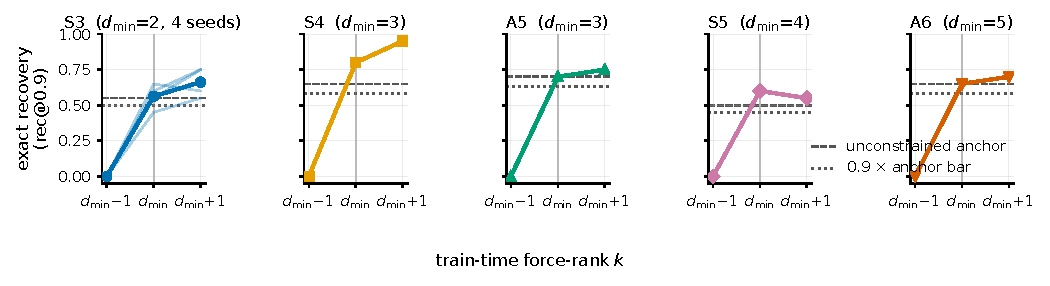
\includegraphics[width=\textwidth]{fig2_razor_step.pdf}
\caption{The converged dimension is causally load-bearing: per group,
crosscheck $\recninety$ on held-out words at train-time force-rank
$k \in \{\dmin{-}1, \dmin, \dmin{+}1\}$ (one seed per cell), vs.\ the
unconstrained anchor (dashed) and the pre-registered $0.9\times$-anchor
bar (dotted). Recovery is exactly 0.000 at $\dmin{-}1$ in every group,
the readout's geometric floor (Appendix~\ref{app:instrument}), and
returns at $\dmin$. $S_3$ overlays its four seeds (thin lines; bold
mean); its below-$\dmin$ zero is unanimous.}
% <!-- evidence: U3 -->
\label{fig:razor}
\end{figure}

Figure~\ref{fig:razor} shows a necessity floor at $\dmin$, not a
plateau. The floor is set by the readout's own geometry, not discovered
by training: $k = \dmin{-}1$ yields $\recninety = 0.000$ in all five
groups
% <!-- evidence: U3 -->
and in all four independent seeds of the $S_3$ extension,
% <!-- evidence: U4 -->
exactly as the bound $\sqrt{(\dmin{-}1)/\dmin} < 0.9$ requires
(Appendix~\ref{app:instrument}); the same cells' recovery cosines
(0.61--0.84) sit under that ceiling, evidence the capped models reached
their rank-constrained optimum rather than collapsing.
% <!-- evidence: U3 -->
Sufficiency is
the empirical result: $S_4$, $A_5$, $S_5$, $A_6$ clear their
pre-registered bars (0.800/0.700/0.600/0.650 against
0.585/0.630/0.450/0.585),
% <!-- evidence: U3 -->
in a majority of groups against a single noisy anchor seed rather than a
stable ceiling, and $S_3$, whose decisive cell landed inside a
pre-stated $\pm 0.05$ marginality trigger, was extended to four seeds
under the trigger's pre-registered routing: the seed-mean (0.5625)
clears the fixed 0.495 bar, though only 2 of 4 seeds individually
(Table~\ref{tab:s3seeds}).
% <!-- evidence: U4 -->
An earlier 58-cell sweep of this grid nulled through an instrument
defect, an ambient identity block in the eye-padded target that taxed
every rank-capped arm;
% <!-- evidence: U6 -->
the verdict was registered as inconclusive with
the tax established from the raw artifacts, and the zero-padded wave
above is the registered fix (Appendix~\ref{app:instrument}).
% <!-- evidence: U6 -->

\section{Related Work and Limitations}
\label{sec:related}

\citet{merrill2024illusion}, \citet{grazzi2025negative}, and
\citet{siems2025deltaproduct} frame state tracking by what recurrent
architectures \emph{can} express on exactly these word problems, the
solvability axis; this work measures what trained states \emph{do}
converge to, and finds the learned dimension sorts by representation
theory instead. \citet{nazari2026rank} and \citet{sun2026staterank}
measure state-rank dynamics in pretrained linear-attention models
observationally, with no algebraic ground truth to converge to and no
causal leg. \citet{nichani2025factual} prove associative-memory capacity
under argmax decoding, the loophole our exact-continuous-recovery
scoring closes; \citet{mishra2026m2rnn} train matrix-state RNNs on $S_3$
composition but measure no state rank and run no rank intervention.
\citet{chughtai2023toy} reverse-engineer which representation-theoretic
structure networks recruit on finite-group composition tasks; this work
asks a narrower question on the same substrate, at what dimension, with
a pre-registered causal intervention absent there.
\citet{huh2024platonic} propose that models trained on different tasks
converge to a shared representation; the present law is a narrower,
algebra-driven instance of that convergence.

\textbf{Limitations.} All results are on sub-1M-parameter synthetic
models under a deliberate single-state bottleneck; nothing here is a
claim about pretrained networks, and the family is five groups with
$\dmin \in \{2,\dots,5\}$ at $\dstate = \dmin + 2$. Causal cells are
single-seed except $S_3$ (four seeds), with the necessity zeros exact
wherever seeds exist; two groups at the shortest pinned budget ($S_3$,
$S_5$) show soft convergence and are also the two with the largest
observational deviation and the one marginal causal cell, a
pre-registered rather than post hoc budget schedule but a caveat on
cross-group comparison strength. The observational readout partially
favors rank $\approx \dmin$ by construction, which is why it was
pre-registered as corroborating and the causal wave carries the claim.


\bibliographystyle{plainnat}
\bibliography{refs}

\appendix

\section{The Five Groups and Reference Representations}
\label{app:groups}

\begin{table}[H]
\centering
\small
\begin{tabular}{lcccl}
\toprule
$G$ & $|G|$ & $\dmin$ & solvable & realization of $\rho_G$ \\
\midrule
$S_3$ & 6   & 2 & yes & standard (dihedral) \\
$S_4$ & 24  & 3 & yes & cube rotations \\
$A_5$ & 60  & 3 & no  & icosahedral rotations \\
$S_5$ & 120 & 4 & no  & standard (zero-sum) \\
$A_6$ & 360 & 5 & no  & standard (zero-sum) \\
\bottomrule
\end{tabular}
\caption{The five task groups. $\dmin$ is the minimal faithful real
representation dimension; each reference representation is orthogonal by
construction and verified faithful (injective on $G$) at build time.
$S_4$/$A_5$ form the designed pair: matched $\dmin$, opposite
solvability.}
\label{tab:groups}
\end{table}

\section{Instrument Details and the Two Defects}
\label{app:instrument}

\textbf{Centering.} For an orthogonal target the uncentered covariance
of $Z(w)$ is isotropic and carries no subspace information; the
production lens centers it (a nontrivial irreducible representation has
zero group mean, cancelling the constant block). The step is
load-bearing: an uncentered lens scores a flawless synthetic model 0.705
where the centered lens scores 0.9996 on identical data.
% <!-- evidence: U7 -->

\textbf{Length-robustness split.} The disclosed split referenced in
Section~\ref{sec:convergence} scores only words of length $L \geq 2$
(the $L = 1$ read is attention-degenerate and was demoted with a
mechanism note in the run records): it moves per-group mean recovery
cosine by at most 0.013 (per-seed at most 0.041), with no
group-selective divergence.
% <!-- evidence: U5 -->

\textbf{The ambient-identity tax.} The first 58-cell sweep's force-rank
target was the eye-padded $\rho_G(\cdot) \oplus I_2$, whose rank is
$\dstate = \dmin + 2$ for every group.
% <!-- evidence: U6 -->
The constant identity block is
the cheapest reliable loss reduction, so a rank-capped arm buys it
first, leaving effective budget $k - 2 < \dmin$ for $\rho_G$ at every
grid point; no capped cell in that sweep ever tested the confirm
direction. The raw-artifact signature: the 39 force-rank cells' direct
cosine matched the rank-$k$ optimum $\sqrt{k/\dstate}$ with mean
absolute deviation 0.028 (maximum 0.166; the two $S_5$ below-$\dmin$
cells are the only outliers, a disclosed optimization shortfall), so the
arms had trained to their rank-constrained ceiling rather than
under-training.
% <!-- evidence: U6 -->
The sweep verdict was registered as inconclusive with the tax as
mechanism; the zero-padded causal wave of Section~\ref{sec:causal} is
the registered fix, its 30 cells configuration-verified one-by-one
against a manifest re-derived independently from the design record. In
that wave an eye-padded corroboration arm reproduces the failure on
demand at raw $k = \dmin{+}1$ (effective budget $\dmin{-}1$) while the
tax-paid point recovers.
% <!-- evidence: U3 -->

\textbf{The observational band's non-binding upper half.}
\texttt{entity\_subspace\_from\_words} returns the top-$\dmin$ left
singular vectors of the centered covariance by construction, so the
restricted state $U^{\top} Z U$ is always $\dmin \times \dmin$, and the
entropy effective rank of a $\dmin \times \dmin$ input has range
$[1, \dmin]$. Restricted effective rank therefore cannot exceed $\dmin$,
and so cannot exceed $1.3 \cdot \dmin$, for any seed of any group; only
the band's lower half, $\geq 0.7 \cdot \dmin$, is a test the data could
fail. Every group mean lands in $[0.895, 0.951] \cdot \dmin$.
% <!-- evidence: U1 -->

\textbf{The rank-constrained cosine ceiling.} The causal wave's target
is $\rho_G(\cdot) \oplus 0$, of rank exactly $\dmin$ with all $\dmin$
informative singular values equal to 1 (the reference representation is
orthogonal by construction, Appendix~\ref{app:groups}). For any matrix
$M$ of rank $\leq k \leq \dmin$, von Neumann's trace inequality gives
$\langle M, T\rangle_F \leq \sum_{i=1}^{k} \sigma_i(M)\,\sigma_i(T) =
\sum_{i=1}^{k} \sigma_i(M)$, and Cauchy--Schwarz bounds
$\sum_{i=1}^{k} \sigma_i(M) \leq \sqrt{k}\,\lVert M \rVert_F$, so
$\cos(M, T) \leq \sqrt{k/\dmin}$. At $k = \dmin{-}1$ this ceiling is
$0.707/0.816/0.816/0.866/0.894$ for $S_3/S_4/A_5/S_5/A_6$, below the
$\recninety$ threshold of 0.9 in every case: no rank-$(\dmin{-}1)$
state, however trained, can register a single word above cosine 0.9
against this target. The necessity result ($\recninety = 0.000$ at
$\dmin{-}1$, all groups, all seeds) is this bound realized, not an
independent discovery about what SGD finds; the corresponding empirical
content is that the observed cosines at $\dmin{-}1$ (0.61--0.84) sit
under their respective rank-constrained optima, evidence optimization
reaches the geometry's own ceiling. At $k \geq \dmin$ the ceiling is
1.0 (exact recovery is representable), so recovery above 0 at $\dmin$
is not guaranteed by the metric and carries the causal weight
(sufficiency).
% <!-- evidence: U3 -->

\textbf{Primary and crosscheck degauging.} The design record's default
pipeline treats scale-only degauging ($\hat{Q} = I$) as the primary
metric, with the fitted-$(c, Q)$ Procrustes score retained as a
robustness cross-check, after calibration on unconstrained checkpoints
found $\hat{Q} \approx I$ empirically. Under the force-rank grid's
zero-padded target this equivalence breaks: the informative block's
degenerate singular spectrum makes the scale-only fit's basis
arbitrary, so the pre-registration for the causal wave specifically
pins the fitted-$(c, Q)$ score, denoted $\recninety$ throughout
Section~\ref{sec:causal} and Figure~\ref{fig:razor}, as decisional; the
scale-only score informs no reported conclusion. The two diverge
sharply on this grid, which is why the distinction is disclosed here.

\section{$S_3$ Per-Seed Causal Detail}
\label{app:s3causal}

\begin{table}[H]
\centering
\small
\begin{tabular}{lcccccc}
\toprule
seed & anchor & $k{=}\dmin{-}1$ & $k{=}\dmin$ & $k{=}\dmin{+}1$ & own bar & clears \\
\midrule
0 & 0.550 & 0.000 & 0.450 & 0.550 & 0.495 & no ($-0.045$) \\
1 & 0.600 & 0.000 & 0.550 & 0.750 & 0.540 & yes ($+0.010$) \\
2 & 0.800 & 0.000 & 0.600 & 0.750 & 0.720 & no ($-0.120$) \\
3 & 0.600 & 0.000 & 0.650 & 0.600 & 0.540 & yes ($+0.110$) \\
\bottomrule
\end{tabular}
\caption{$S_3$ four-seed causal detail (crosscheck $\recninety$) behind
the seed-mean confirmation in Section~\ref{sec:causal}; the own bar is
$0.9 \times$ each seed's anchor. $k = \dmin{-}1$ reads exactly 0.000 in
all four seeds; $k = \dmin$ clears each seed's own bar in 2 of 4 (seeds
1, 3), missing in the other 2 because the anchor itself ranges
0.550--0.800 across seeds. The pre-registered criterion compares the
seed-mean $k = \dmin$ value (0.5625) against the bar fixed before the
extension ran (0.495, from seed 0's anchor), specifically to avoid
computing the bar from the same noisy seeds it is judged against;
recomputing the bar as $0.9\times$ the four-seed anchor mean (raw mean
0.6375, bar 0.574) would put the seed-mean value 0.011 below it.}
% <!-- evidence: U4 -->
\label{tab:s3seeds}
\end{table}

\section{Per-Seed Observational Rank}
\label{app:m1}

\begin{table}[H]
\centering
\small
\begin{tabular}{lccccc}
\toprule
$G$ & $\dmin$ & $n$ & restricted eff.\ rank & band & in band \\
\midrule
$S_3$ & 2 & 3 & $1.877 \pm 0.060$ & $[1.4, 2.6]$ & 3/3 \\
$S_4$ & 3 & 5 & $2.852 \pm 0.054$ & $[2.1, 3.9]$ & 5/5 \\
$A_5$ & 3 & 5 & $2.832 \pm 0.062$ & $[2.1, 3.9]$ & 5/5 \\
$S_5$ & 4 & 3 & $3.591 \pm 0.069$ & $[2.8, 5.2]$ & 3/3 \\
$A_6$ & 5 & 3 & $4.736 \pm 0.023$ & $[3.5, 6.5]$ & 3/3 \\
\bottomrule
\end{tabular}
\caption{Restricted effective rank of the unconstrained trained state
(mean $\pm$ sd over seeds) against each group's $\dmin$, with the
pre-registered $[0.7, 1.3] \cdot \dmin$ band. Every seed of every group
is in band; Spearman $\rho = 0.9747$ is the tie-capped maximum; the
dimension-matched pair $S_4$/$A_5$ differs by 0.019 rank-units.}
% <!-- evidence: U1 -->
\label{tab:m1}
\end{table}


\end{document}
